%\motto{Use the template \emph{chapter.tex} to style the various elements of your chapter content.}
\chapter{Medizinische Anwendungsgebiete}
\label{trends} % Always give a unique label
% use \chaptermark{}
% to alter or adjust the chapter heading in the running head

\chapterauthor{Martin Maier, Siri Wandel}

\abstract{some abstract}

\section{Relevanz \& Problemstellung}
Die Medizin und Pharmaindustrie stehen vor großen Herausforderungen, die Innovation erfordern, um die Entwicklung neuer Medikamente zu beschleunigen und Behandlungsmethoden zu verbessern. Gleichzeitig steigen die Anforderungen an personalisierte Medizin, die präzisere Diagnostik und die schnellere Reaktion auf neue Krankheitsausbrüche, wie COVID-19. Trotz fortschrittlicher Rechenmodelle und Big Data Ansätzen, welche Kostenreduktionen in der Medikamentenentwicklung versprechen, stoßen klassische Computer an physikalische und mathematische Grenzen, hier eröffnet Quanteninformatik neue Horizonte. (Vgl. \cite{blunt_perspective_2022}; \cite{shweta_quantum_2024}) Dies könnte einen Paradigmenwechsel in der Art und Weise, wie wir medizinische Forschung betreiben, ermöglichen.\\
\\
Die Entwicklung neuer Medikamente nimmt einen Zeitraum zwischen 5 und 20 Jahren oft mehr als ein Jahrzehnt in Anspruch, verursacht Kosten in Milliardenhöhe und ist mit einer hohen Misserfolgsquote verbunden. Dieser Prozess könnte mithilfe von Quantum Computing beispielsweise durch die Simulation von Molekülstrukturen beschleunigt und ermöglicht werden. Somit könnten Wechselwirkungen zwischen Medikamenten und Proteinen genauer vorhergesagt und optimiert werden. Das könnte eine Reduktion der Entwicklungszeit, sowie der damit verbundenen Kosten zur Folge haben. (Vgl. \cite{brown_clinical_2022}; \cite{schlander_how_2021}; \cite{shweta_quantum_2024})\\
\\
Weitere Probleme in der Medizin- und Pharmaindustrie liegen unter anderem in der Erstellung von personalisierten Therapie- und Behandlungsplänen, der Sicherung von Patientendaten, innerhalb der medizinischen Bildgebung oder auch der Entschlüsselung des menschlichen Genoms. (Vgl. \cite{shweta_quantum_2024}) Grundsätzlich besteht ein großes Potenzial in Bezug auf die Nutzung von Quantum Computing in der Medizin- und Pharmaindustrie. Trotz des großen Potenzials gibt es jedoch noch erhebliche Herausforderungen zu bewältigen. Begrenztes Fachwissen und begrenzte Hard- und Softwarelösungen zählen dabei zu den Hauptherausforderungen.


\section{Top 3 Anwendungsfelder (Praxis \& Theorie)}
\label{med:applicationFields}
Die potenziellen Einsatzmöglichkeiten von Quantencomputern im Gesundheitswesen sind vielfältig, wie Abbildung \ref{fig:use-cases-medicine} verdeutlicht. Sie reichen von molekularer Simulation über Krebsbehandlung bis hin zu Bildanalyseverfahren. In diesem Abschnitt liegt der Fokus auf den drei Anwendungsfeldern, die aktuell sowohl in der Forschung als auch in der industriellen Entwicklung eine herausragende Rolle spielen: Wirkstoffentwicklung, Proteinstrukturvorhersage und Personalisierte Medizin.\\
\\
\begin{figure}[ht]
    \centering
    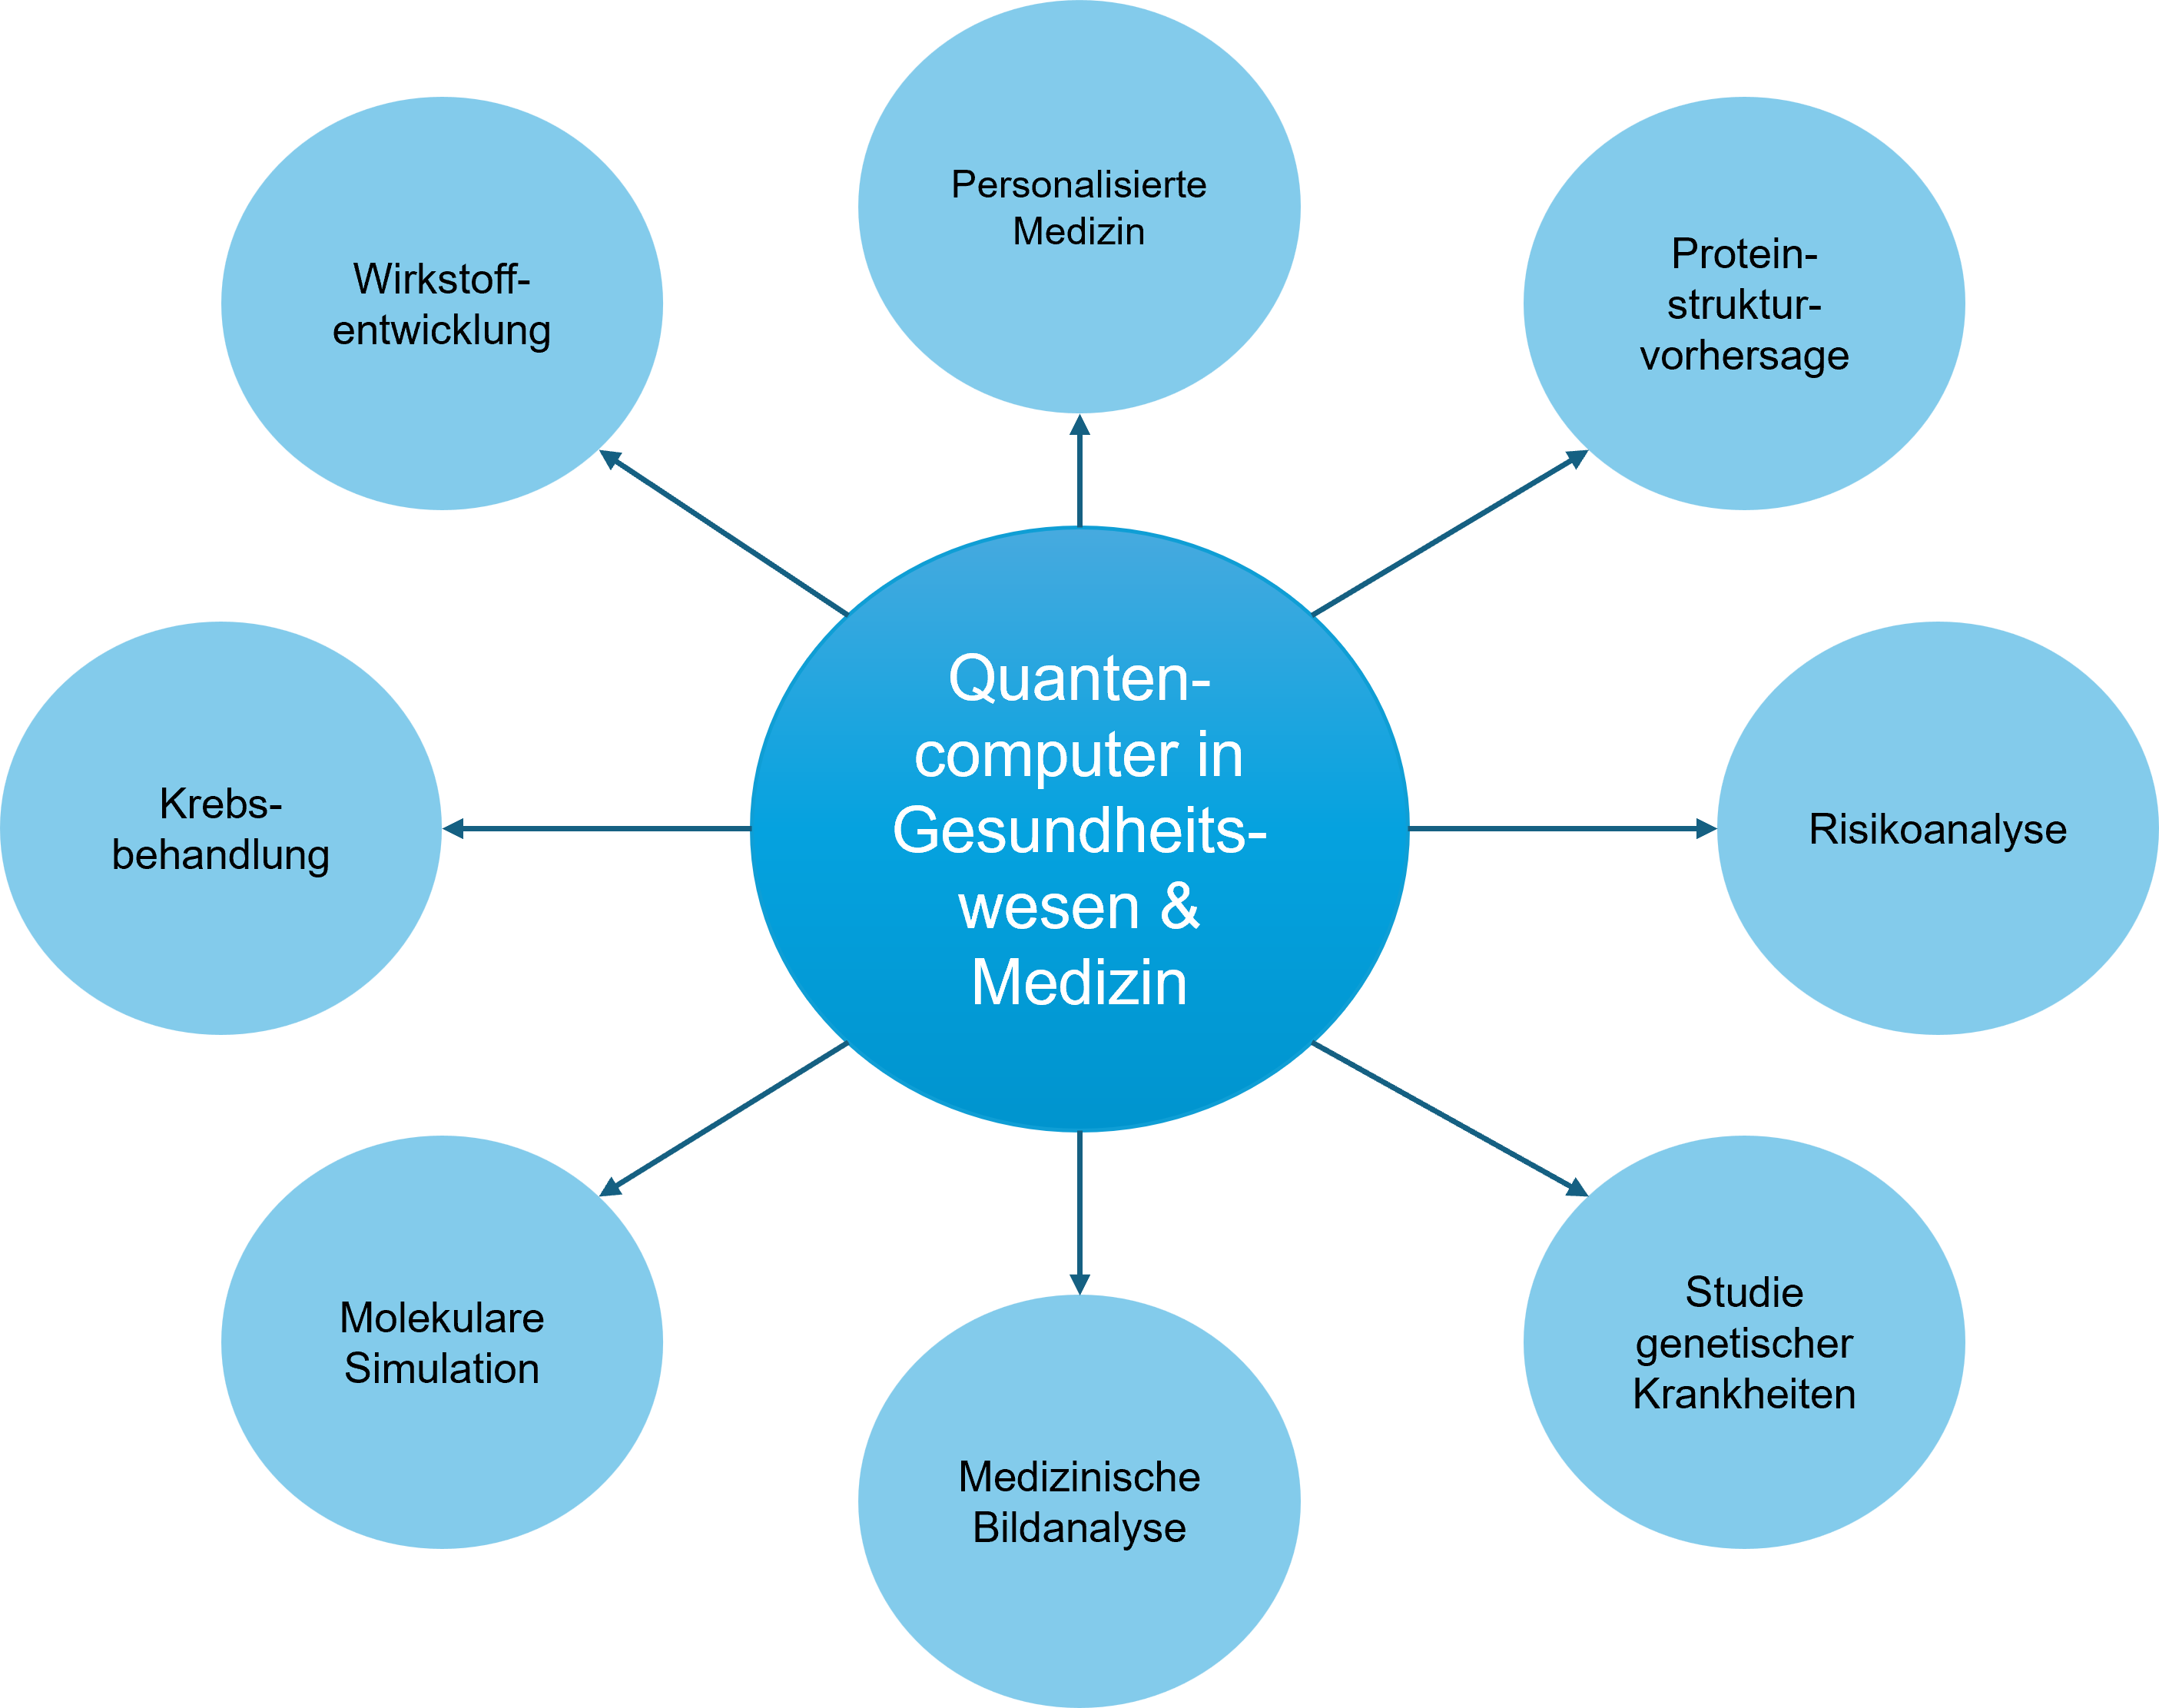
\includegraphics[width=.8\textwidth]{images/medicine/AnwendungsfelderMedizin.png}
    \caption{Übersicht möglicher Einsatzfelder von Quantencomputern in der Medizin. (Eigene Darstellung nach \cite{dhande_quantum_2023}.)}
    \label{fig:use-cases-medicine}
\end{figure}
\\
Diese Auswahl basiert auf drei qualitativen Kriterien: Erstens adressieren diese Bereiche relevante medizinische Herausforderungen. Zweitens zeichnen sie sich durch eine besonders hohe rechnerische Komplexität aus, die den Einsatz von Quantencomputern sinnvoll erscheinen lässt. Drittens bestehen bereits erste praxisnahe Anwendungen und Pilotprojekte, die eine Brücke zwischen theoretischem Potenzial und konkreter Nutzung bilden. Die Auswahl orientiert sich somit nicht nur an theoretischem Potenzial, sondern auch an praktischer Umsetzbarkeit und gesellschaftlicher Relevanz.

\subsection{Wirkstoffentwicklung}
Die Entwicklung neuer Wirkstoffe ist grundlegend mit hohen Kosten verbunden. Das liegt besonders an langen Entwicklungszyklen und einer geringen Erfolgsquote. Der Einsatz von Computern, besonders im Rahmen des Computer"=Aided Drug Design (CADD), ist in der pharmazeutischen Forschung etabliert. Dies stößt jedoch bei der Modellierung komplexer molekularer Systeme an seine Grenzen (Vgl. \cite{bertl_quantum_2025}).\\
\\
Ein wichtiger Einsatzbereich von Quantencomputern in der Wirkstoffentwicklung ist die präzise Berechnung molekularer Eigenschaften. Besonders relevant sind hier der Variational Quantum Eigensolver (VQE) und die Quantum Phase Estimation (QPE). Diese Algorithmen werden genutzt, um die Schrödinger-Gleichung für Moleküle zu lösen. Damit lassen sich elektronische Strukturen, Energiezustände oder Bindungseigenschaften genauer bestimmen. Das ist zentral, um zu verstehen, wie ein Wirkstoff mit seinem Ziel im Körper interagiert. Ergänzend dazu kommen weitere Methoden zum Einsatz. Quantum Machine Learning (QML) kann molekulare Eigenschaften auf Basis quantenmechanischer Daten vorhersagen oder helfen, Wirkstoffkandidaten gezielt zu verbessern. Quantum Annealing eignet sich gut für Optimierungsprobleme, zum Beispiel um stabile Molekülkonfigurationen mit starker Zielbindung zu finden. Auch Prozesse wie die Aufnahme, Verteilung und Wirkung eines Medikaments im Körper, also Pharmakokinetik und Pharmakodynamik, lassen sich mit Quantenmodellen realistischer simulieren. So kann Quantencomputing an verschiedenen Stellen der Wirkstoffentwicklung unterstützen. (Vgl. \cite{bertl_quantum_2025})

\subsubsection*{Compound Screening \& Lead"=Optimierung}
Quantencomputer versprechen, diese Prozesse durch genauere und schnellere Simulationen von Molekülen und deren Wechselwirkungen erheblich zu verbessern. Dabei konzentrieren sich aktuelle Quantencomputing"=Anwendungen in der pharmazeutischen Forschung besonders auf zwei frühe Phasen der Wirkstoffentwicklung: das \textit{Compound Screening} und die \textit{Lead"=Optimierung}. Beim Compound Screening werden sehr viele verschiedene chemische Verbindungen daraufhin untersucht, ob sie grundsätzlich an ein Zielmolekül (z.B. ein krankheitsrelevantes Protein) binden können. In der Lead"=Optimierung werden dann vielversprechende Kandidaten gezielt verbessert, um deren Wirksamkeit und Verträglichkeit zu steigern. Quantencomputer können in diesen Phasen helfen, indem sie Wechselwirkungen zwischen Molekülen genauer simulieren und energetisch günstige Strukturen besser vorhersagen (Vgl. \cite{zinner_quantum_2021}).

\subsubsection*{Quantenchemische Simulation}
Auf theoretischer Ebene gilt die quantenchemische Berechnung von Molekül"=Energien als eines der vielversprechendsten Anwendungsfelder des Quantencomputings. Sie ist essenziell für die Ermittlung von Bindungsaffinitäten, Reaktionspfaden und energetisch bevorzugten Konformationen, welche zentrale Größen in der computergestützten Wirkstoffentwicklung sind. Wie \cite{cao_quantum_2019} betonen: Das klassische Problem, dessen Lösung vom Quantencomputing erwartet wird, ist die Berechnung von Grundzustands- und angeregten Zustandsenergien kleiner Moleküle. Solche Berechnungen dienen als Ausgangspunkt für die Bestimmung vieler nützlicher Größen, wie etwa Reaktionspfaden, Bindungsenergien und Reaktionsgeschwindigkeiten chemischer Prozesse. (eigene Übersetzung nach \cite{cao_quantum_2019}.) Zentral ist demnach die Berechnung von Molekülenergien, da sie viele wichtige chemische Eigenschaften bestimmt.

\subsubsection*{Virtuelles Screening und datengetriebene Modellierung}
Beim \textit{virtuellen Screening} handelt es sich um einen frühen Schritt im Prozess der Wirkstoffentwicklung. Dabei werden mit Hilfe von Computern große Datenbanken nach Molekülen durchsucht, die an ein bestimmtes krankheitsrelevantes Ziel binden könnten. So lassen sich vielversprechende Wirkstoffkandidaten schneller finden und unnötige Labortests vermeiden. Klassische Methoden stoßen dabei aber oft an Grenzen: Die Modelle sind manchmal ungenau, liefern viele falsche Treffer und brauchen viel Rechenleistung. Neue Ansätze wie Quantum Machine Learning können hier helfen. Mit Quantencomputern lassen sich Molekülwechselwirkungen genauer simulieren und komplexe Daten effizienter verarbeiten. Techniken wie Quanten"=Neuronale Netzwerke, Quanten"=Kernel oder spezielle Quanten"=Suchalgorithmen ermöglichen ein gezielteres und schnelleres Screening. (Vgl. \cite{kumar_recent_2024})


\subsection{Proteinstrukturvorhersage}
\label{med:protein}
Die bisher etablierten Methoden zur Proteinstrukturvorhersage haben bereits beeindruckende Fortschritte erzielt. Mit experimentellen Ansätzen sowie durch KI"=basierte Modelle wie AlphaFold, RoseTTaFold und verwandte Systeme lassen sich für viele Proteine dreidimensionale Strukturen bereits mit hoher Genauigkeit vorhersagen. (Vgl. \cite{jumperHighlyAccurateProtein2021}; \cite{baekAccuratePredictionProtein2021})\\
\\
Besonders relevant ist dabei der VQE, der in hybriden Verfahren genutzt wird, um energiearme Faltungskonfigurationen zu berechnen. Auch quantumbasierte Optimierungsansätze auf Gittermodellen spielen eine Rolle, da sie es erlauben, Faltungsprozesse vereinfacht, aber physikalisch fundiert zu simulieren. Diese Algorithmen bieten eine Alternative zu klassischen Methoden, die bei komplexen oder künstlichen Proteinsequenzen oft an ihre Grenzen stoßen. (Vgl. \cite{doga_perspective_2024}; \cite{robert_resource-efficient_2021})

\subsubsection*{Grenzen klassischer Methoden}
Diese klassischen Methoden basieren meist auf Mustern aus bekannten Proteinstrukturen und liefern häufig nur ein begrenztes Verständnis der physikalischen Prozesse, die der Proteinfaltung zugrunde liegen. Das erschwert insbesondere die Vorhersage bei synthetischen oder stark abweichenden Aminosäuresequenzen. Studien zeigen, dass Modelle wie AlphaFold2 bei solchen Sequenzen außerhalb ihres Trainingsdatensatzes unzuverlässige Ergebnisse liefern können (Vgl. \cite{outeiralCurrentStructurePredictors2022}). Physikbasierte Verfahren wie die Molekulardynamik bieten zwar grundsätzlich eine höhere Genauigkeit, sind jedoch für größere Proteine extrem rechenintensiv und in der Praxis kaum skalierbar (Vgl. \cite{doga_perspective_2024}). Diese Einschränkungen verdeutlichen den Bedarf an alternativen Modellierungsansätzen.

\subsubsection*{Quantenbasierte Faltungsmodelle}
Quantencomputer könnten eine vielversprechende Alternative bieten, da sie durch Quantenparallelismus potenziell viele Faltungszustände gleichzeitig analysieren können (Vgl. \cite{doga_perspective_2024}). Aktuelle Forschungsarbeiten formulieren die Proteinfaltung dabei als Optimierungsproblem und setzen auf Quantenalgorithmen sowie vereinfachte physikalische Modelle. Zwei Ansätze haben sich dabei als besonders vielversprechend erwiesen: Hybridverfahren mit VQE und quantenbasierte Gittermodelle.\\
\\
Im Ansatz von \citeauthor{doga_perspective_2024} wurde ein hybrider Algorithmus eingesetzt, der klassische Optimierung mit einem VQE kombiniert. Ziel war die Vorhersage der Struktur eines kurzen Abschnitts mit sieben Aminosäuren aus dem Helikaseprotein des Zika"=Virus. Solche Abschnitte werden als Loops bezeichnet. Sie verbinden regelmäßige Strukturelemente wie Alpha"=Helices und Beta"=Faltblätter und sind häufig entscheidend für die Funktion eines Proteins. Die räumliche Anordnung der Atome in diesem Abschnitt, also die sogenannte Konformation, wurde anschließend mit bekannten Referenzdaten verglichen. Die mittels Quantencomputer berechnete Struktur wich deutlich weniger vom experimentell bestimmten Referenzmodell ab als die Vorhersage von AlphaFold2. Der mittlere Abstand der Atome (RMSD) betrug etwa 1,88 Å bei der Quantenmethode und 3,53 Å bei AlphaFold2. Das zeigt, dass quantenbasierte Verfahren bereits heute genauere Ergebnisse liefern können als etablierte KI"=Modelle. Zumindest für kleinere, aber strukturell anspruchsvolle Proteinbereiche. (Vgl. \cite{doga_perspective_2024})\\
\\
Ein weiterer Ansatz basiert auf Gittermodellen. \citeauthor{robert_resource-efficient_2021} verwendeten ein solches Modell zur Faltung kurzer Peptide mit IBM-Quantenhardware. Ein 10"=Aminosäure"=Peptid (Angiotensin) wurde auf 22 Qubits, ein 7-Aminosäure-Peptid auf 9 Qubits kodiert. Die Ergebnisse zeigen, dass selbst kleine Quantencomputer bereits in der Lage sind, realistische Faltungskonfigurationen effizient zu berechnen. (Vgl. \cite{robert_resource-efficient_2021})


\subsection{Personalisierte Medizin}
Die personalisierte Medizin verfolgt das Ziel, medizinische Entscheidungen stärker an den individuellen Eigenschaften eines Patienten auszurichten, etwa an genetischen Merkmalen, Krankheitsverläufen oder Therapieansprechen. Das bedeutet, dass aus komplexen, oft hochdimensionalen Daten wie Genomsequenzen, Laborwerten oder Bilddaten präzise Vorhersagen abzuleiten sind. Klassische Methoden stoßen hierbei zunehmend an ihre Grenzen, insbesondere bei kleinen Datensätzen, hoher Variabilität oder stark nichtlinearen Zusammenhängen. Auch maschinelles Lernen stoßt bei individuellen oder seltenen Fällen oft an seine Grenzen. Bei wenigen Trainingsdaten führen sie zu unsicheren Diagnosen und Therapieentscheidungen. (Vgl. \cite{gupta_systematic_2025}).\\
\\
Einige Algorithmen spielen in der personalisierten Medizin eine besonders wichtige Rolle. QML und QNN eignen sich, um individuelle Krankheitsverläufe und Therapieantworten vorherzusagen. Erste Studien zeigen, dass sich damit zum Beispiel Tumordynamiken modellieren oder Therapieergebnisse besser abschätzen lassen. Ergänzend werden QAOA und VQA eingesetzt, etwa zur Planung klinischer Studien oder zur Auswahl geeigneter Patientengruppen. Auch generative Modelle wie Quantum Boltzmann Machines finden Anwendung, etwa zur Erzeugung synthetischer Patientendaten. Diese Methoden erweitern die Möglichkeiten klassischer Verfahren, ohne sie vollständig zu ersetzen. (Vgl. \cite{bertl_quantum_2025})

\subsubsection*{P5"=Medizin}
In der aktuellen Forschung wird personalisierte Medizin zunehmend als sogenanntes P5"=Modell verstanden. Dieses erweitert das bisherige P4"=Modell um eine fünfte Dimension: \textit{psychokognitiv}. Die fünf Elemente lauten: vorhersagend (predictive), vorbeugend (preventive), personalisiert, beteiligend (participatory) und psychokognitiv. Letztere betont psychologische und kognitive Faktoren wie Werte, Lebensqualität und Gesundheitskompetenz. Diese beeinflussen, wie Patienten mit Erkrankungen umgehen und wie sie auf Therapien reagieren. (Vgl. \cite{gorini_p5_2011})\\
\\
Quantencomputing kann in diesem Kontext neue Wege eröffnen. Durch seine Fähigkeit, viele Datenmuster gleichzeitig zu analysieren, lassen sich verhaltensbezogene Einflussfaktoren stärker in personalisierte Modelle integrieren. Besonders vielversprechend ist hier der Einsatz von Quantum Machine Learning, also von Modellen, die klassische Lernverfahren mit quantenmechanischen Elementen kombinieren (Vgl. \cite{bertl_quantum_2025}.)

\subsubsection*{Frühe Anwendungen von Quantum Machine Learning}
Eine aktuelle Übersichtsarbeit zeigt, dass sich erste klinisch relevante QML-Anwendungen zum Beispiel in der EKG"=Analyse, Genomik oder Bildgebung bereits auf echter Quantenhardware testen lassen, wenn auch bisher in begrenztem Umfang (Vgl. \cite{gupta_systematic_2025}). Besonders Genomik und Bildgebung ermöglichen eine präzisere Diagnostik und auf individuelle genetische Profile abgestimmte Therapieansätze. Ein konkretes Beispiel liefert eine Studie zur Vorhersage von Arzneimittelwirkungen bei Krebspatienten. In dieser erzielt ein hybrides QNN eine bis zu 15 Prozent höhere Genauigkeit als klassische Modelle, bei signifikant kürzerer Trainingszeit (Vgl. \cite{sagingalieva_hybrid_2023}).\\
\\
\begin{table}[ht]
\centering
\renewcommand{\arraystretch}{1.3}
\resizebox{\textwidth}{!}{
\begin{tabular}{|p{2.3cm}|p{4.5cm}|p{2.5cm}|p{4.5cm}|}
\hline
\textbf{Anwendungsfeld} & \textbf{Rechnerische Herausforderung} & \textbf{Quantenansatz / Algorithmus} & \textbf{Warum QC relevant?} \\
\hline
Drug Discovery & Molekül-Energieberechnung, Bindungsaffinitäten & VQE, QPE & Klassische Methoden zu ungenau oder zu langsam \\
\hline
Proteinstruktur & Kombinatorische Explosion möglicher Faltungen & QAOA, Hybridalgorithmen & QC kann Zustände simultan analysieren \\
\hline
Personalisierte Medizin & Mustererkennung in hochdimensionalen Daten & QML, QNN & Klassische Modelle überfordert bei komplexer Nichtlinearität \\
\hline
\end{tabular}
}
\caption{Anwendungsfelder des Quantencomputings in der Medizin und Pharmazie}
\label{tab:qc_medizin}
\end{table}
\\


\section{Top Technologien \& Algorithmen}

\subsection{Variational Quantum Eigensolver (VQE)}
Der Variational Quantum Eigensolver (VQE) ist ein Algorithmus zur Lösung quantenchemischer Probleme und findet zunehmend Anwendung im medizinischen Kontext. In der quantenchemischen Simulation kann VQE genutzt werden, um Molekülenergien, Bindungsaffinitäten und Reaktionspfade zu berechnen. Diese Größen sind entscheidend für die Beurteilung chemischer Stabilität und Reaktivität und spielen eine wichtige Rolle bei der frühen Identifikation potenzieller Wirkstoffe (Vgl. \cite{palFuturePotentialQuantum2024}; \cite{cao_quantum_2019}). Darüber hinaus wird VQE auch in der Strukturbiologie erforscht. Er kann eingesetzt werden, um die Energie von Proteinbausteinen oder Ligand-Protein-Komplexen abzuschätzen, was dazu beiträgt, molekulare Wechselwirkungen besser zu verstehen (\cite{marchettiQuantumComputingAlgorithms2022}). Studien deuten zudem darauf hin, dass VQE künftig auch für die Simulation individueller Stoffwechselprozesse genutzt werden könnte. Dies betrifft beispielsweise Anwendungen in der personalisierten Medizin, etwa zur Vorhersage individueller Therapieerfolge oder bei der Entwicklung neuer Kontrastmittel für bildgebende Verfahren (\cite{palFuturePotentialQuantum2024}).

\subsection{Quantum Phase Estimation (QPE)}
Der Quantum Phase Estimation (QPE) Algorithmus gilt als zentrale Methode zur präzisen Bestimmung von Grundzustandsenergien von Molekülen und ist damit von besonderem Interesse für die Wirkstoffentwicklung, etwa bei pharmazeutisch relevanten Substanzen wie Ibrutinib. Im Vergleich zu klassischen Verfahren bietet QPE das Potenzial für eine exponentielle Beschleunigung solcher Berechnungen. Die herkömmliche Lehrbuchvariante von QPE ist jedoch sehr ressourcenintensiv und anfällig für Fehler, da sie zahlreiche Hilfs-Qubits und tiefe Schaltkreise erfordert. Um diese Limitierungen zu überwinden, wurden speziell für frühe fehlertolerante Quantencomputer (EFTQCs) optimierte Protokolle wie Iterative Phase Estimation (IPE), Robust Phase Estimation (RPE), Quantum Complex Exponential Least Squares (QCELS) und Multi"=Modal Multi"=Level QCELS (MMQCELS) entwickelt. Diese reduzieren sowohl die Zahl der benötigten Ancilla"=Qubits als auch die Schaltungstiefe und verbessern die Robustheit gegenüber Fehlern deutlich. Studien zeigen, dass das Berechnungsvolumen im Vergleich zur klassischen QPE um ein Vielfaches gesenkt werden kann. Teilweise um das bis zu 300-Fache. Ergänzend leisten Fortschritte in der Optimierung der Simulationstechniken und der Fehlerminderung einen Beitrag zur praktischen Umsetzbarkeit dieser Methoden. (Vgl. \cite{nelson_assessment_2024}; \cite{blunt_perspective_2022}; \cite{blunt_statistical_2023})

\subsection{Quantum Approximate Optimization Algorithm (QAOA)}
QAOA ist ein variationaler Quantenalgorithmus zur näherungsweisen Lösung kombinatorischer Optimierungsprobleme, der im medizinischen Bereich insbesondere in der Proteinfaltung und im molekularen Docking Anwendung findet. Für das Proteinfaltungsproblem wurde QAOA in vereinfachten Gittermodellen getestet, wobei es energiearme Konformationen mit höherer Wahrscheinlichkeit erzeugen konnte als rein zufälliges Sampling. Allerdings erfordern realistischere Modelle deutlich tiefere Quantenschaltkreise, was eine Anwendung auf atomarer Ebene derzeit noch erschwert. Größeres Potenzial zeigt QAOA im Bereich des molekularen Dockings, das für die Entwicklung neuer Medikamente zentral ist. Durch die Formulierung des Problems als maximal gewichtete Clique lassen sich mit dem verbesserten DC"=QAOA"=Ansatz biologisch relevante Bindungsstellen effizienter identifizieren. Fallstudien mit relevanten Zielproteinen wie SARS"=CoV"=2 Mpro, DPP-4 und HIV-1 gp120 belegen eine hohe Übereinstimmung mit bekannten Strukturen. Gleichzeitig zeigt DC"=QAOA Vorteile bei der Ressourcennutzung, da es weniger Gatter und Iterationen benötigt als klassische Varianten. Herausforderungen bestehen weiterhin in der Stabilität der Optimierung, insbesondere bei komplexeren molekularen Systemen. (Vgl. \cite{ding_molecular_2024}; \cite{boulebnane_peptide_2023})

\subsection{Hybride Quantenklassische Algorithmen}
Hybride quantenklassische Algorithmen kombinieren klassische Rechenmethoden mit quantenmechanischen Komponenten und gelten als vielversprechender Ansatz für medizinische Anwendungen im Zeitalter begrenzter Quantenhardware. Besonders in der personalisierten Medizin und Wirkstoffentwicklung zeigen sich erste sinnvolle Einsatzmöglichkeiten. So lassen sich etwa Biomarker für bestimmte Krebsarten wie das klarzellige Nierenzellkarzinom genauer klassifizieren, was die Diagnose verbessern und Therapien gezielter ermöglichen kann. Auch in der computergestützten Entwicklung neuer Medikamente bieten hybride Verfahren Vorteile, zum Beispiel bei der Simulation chemischer Bindungen oder der Bewertung pharmakologisch relevanter Energieprofile. Diese Ansätze verdeutlichen, dass sich Quantencomputing bereits heute sinnvoll mit bestehenden Methoden verknüpfen lässt, um medizinische Entscheidungsprozesse zu unterstützen. (Vgl. \cite{li_hybrid_2024}; \cite{astuti_use_2025})

\subsection{Quantum Machine Learning (QML) \& Quantum Neural Networks (QNN)}
Quanten-Maschinelles Lernen (QML) und Quanten-Neuronale Netzwerke (QNN) sind speziell entwickelte Quantenalgorithmen zur Analyse klassischer Gesundheitsdaten. Insbesondere im Zuge der zunehmenden Digitalisierung, etwa durch elektronische Gesundheitsakten, gelten sie als vielversprechende Werkzeuge für klinische Entscheidungshilfen, Gesundheitsprognosen und kontinuierliches Monitoring. QNNs kommen dabei als gate-basierte Modelle zum Einsatz, die sich gezielt für solche Aufgaben einsetzen lassen. Eine systematische Übersichtsarbeit zu Veröffentlichungen zwischen 2015 und 2024 zeigt jedoch, dass es bislang an empirischer Evidenz für einen klaren Vorteil gegenüber klassischen Verfahren mangelt. Die meisten Studien konzentrierten sich auf Diagnose- und Prognoseanwendungen, während wichtige Bereiche wie Public Health oder Versorgungsforschung kaum berücksichtigt wurden. Darüber hinaus erfolgten viele Untersuchungen unter idealisierten Bedingungen und setzten vereinfachte, lineare Modelle ein, ohne reale Fehlerquellen zu integrieren. (Vgl. \cite{gupta_systematic_2025})

\subsection{Technologische Frameworks}
Die in diesem Abschnitt vorgestellten technologischen Frameworks orientieren sich an den in Kapitel \ref{med:applicationFields} beschriebenen Anwendungsfeldern. Ziel ist es, die eingesetzten Softwarestacks und Entwicklungstools entlang ihrer praktischen Einsatzbereiche in der Wirkstoffentwicklung, der Proteinstrukturvorhersage und der personalisierten Medizin systematisch darzustellen. Auf diese Weise wird deutlich, wie spezifische Quantenalgorithmen in den jeweiligen medizinischen Kontexten technologisch implementiert werden.\\

\subsubsection*{Wirkstoffentwicklung}
Die praktische Umsetzung der Quantenalgorithmen für medizinische Anwendungen erfordert leistungsfähige Software"=Stacks, die Quanten-Hardware und klassische Algorithmen verbinden. Für die Wirkstoffentwicklung werden vor allem Frameworks genutzt, die komplexe \textit{Molekül"=Hamilton"=Operatoren} bearbeiten und Verfahren wie VQE oder QPE effizient implementieren. Bei den Operatoren handelt es sich um mathematische Ausdrücke, die alle relevanten physikalischen Eigenschaften eines Moleküls quantenmechanisch beschreiben. Der Hamilton"=Operator bildet somit die Grundlage für die Simulation von Molekülzuständen, da er die Energieverteilung eines Systems vollständig bestimmt (Vgl. \cite{mcardle_quantum_2020}).\\
\\
So bietet IBM Qiskit mit dem Qiskit Nature"=Modul spezialisierte Werkzeuge zur Darstellung chemischer Systeme und zum Lösen von Grundzustandsproblemen in Molekülen (Vgl. \cite{developers_qiskit_2023}). Microsofts Q\# Quantum Development Kit (QDK) enthält ebenfalls eine Chemie-Bibliothek mit qubitisierten Fermionen-Operatoren sowie Implementierungen von Hamilton-Simulatoren (Trotterisierung, Qubitierung) (Vgl. \cite{team_simulating_2018}). \\
\\
Amazon Braket ist ein vollständig verwalteter Cloud-Dienst von AWS, der es Forscherinnen und Forschern ermöglicht, Quantenalgorithmen zu entwerfen, auf verschiedenen Simulatoren zu testen und auf realen Quantencomputern auszuführen. Damit bietet Braket eine flexible Entwicklungsumgebung für hybride quantenklassische Workflows in der Arzneimittelforschung. Besonders relevant für medizinische Anwendungen ist der Zugriff auf unterschiedliche Hardwareplattformen innerhalb eines einheitlichen SDK. Braket unterstützt unter anderem gatterbasierte Quantencomputer von IonQ, IQM und Rigetti sowie einen Analog Hamiltonian Simulator (AHS) von QuEra. Letzterer erlaubt die direkte Simulation physikalischer Systeme auf Basis kontinuierlicher Hamilton-Operatoren, was für bestimmte molekulare Strukturberechnungen von Vorteil sein kann (Vgl. \cite{noauthor_quantum_nodate-1}). Dieser flexible Ansatz wird beispielsweise im AWS"=Toolkit QCEDD genutzt, das eingebaute Beispiele für Aufgaben wie molekulares Docking und Faltungsprobleme in der Wirkstoffforschung enthält. (Vgl. \cite{noauthor_quantum_nodate})\\ %evtl. git repo zitieren

%besonders beim virtuellen screening relevant 

\subsubsection*{Proteinstrukturvorhersage}
Die Vorhersage von Proteinstrukturen ist ein hochdimensionales Optimierungsproblem. Klassischerweise modelliert man Proteine auf Gitternetzen, um die Konformationsräume lösbar zu machen. Wie bereits in Kapitel \ref{med:protein} dargelegt, sind Quantenoptimierungsalgorithmen wie QAOA dafür gut geeignet. (Vgl. \cite{boulebnane_peptide_2023})\\
\\
Zur praktischen Umsetzung von Algorithmen wie QAOA in der Proteinstrukturvorhersage wird geeignete Software benötigt, die die Komplexität quantenmechanischer Optimierung handhabbar macht. Ein bekanntes Framework in diesem Bereich ist \textit{PennyLane}. Es ist eine plattformunabhängige Open"=Source"=Bibliothek für Quantencomputing und Quantum Machine Learning, die für wissenschaftliche Anwendungen entwickelt wurde. Durch PennyLane können Quantenalgorithmen mit klassischen Lernverfahren kombiniert werden. Das ist besonders bei der Proteinstrukturvorhersage von Vorteil, da hier sowohl quantenbasierte Optimierung, als auch klassische Auswertungsverfahren erforderlich sind. (Vgl. \cite{noauthor_what_nodate})\\
\\
Das Start"=up Menten AI nutzt PennyLane für die Entwicklung neuer proteinbasierter Wirkstoffe. Ziel ist es, Quantencomputing und klassische Verfahren so zu kombinieren, dass neue Wirkstoffkandidaten schneller und gezielter gefunden werden können. Dabei setzt Menten AI auf PennyLane, um Quantenalgorithmen effizient einzubinden und bioaktive Peptide für neue Therapien zu entwickeln. Das heißt, sie nutzen die Software, um schneller passende Wirkstoffe zu finden, die gut an bestimmte Krankheitsziele andocken können. (Vgl. \cite{abdel-kareemXanaduUSAir2025})\\

\subsubsection*{Personalisierte Medizin}
In der personalisierten Medizin stehen große und komplexe Datensätze im Fokus, zum Beispiel aus Genomik, Bildgebung oder klinischen Untersuchungen. Um diese besser auszuwerten, werden zunehmend Frameworks genutzt, die klassische Machine"=Learning"=Modelle mit Quantenkomponenten verbinden. Ein wichtiges Beispiel ist \textit{TensorFlow Quantum}, das das Quantenframework \textit{Cirq} mit dem bekannten Lernframework \textit{TensorFlow} kombiniert. Es ermöglicht hybride Modelle, bei denen klassische und quantenbasierte Rechenschritte gemeinsam genutzt werden. Das ist besonders relevant, da Quantenprozessoren aktuell noch fehleranfällig und begrenzt einsetzbar sind. Durch die Kombination mit klassischen Prozessoren kann das Potenzial von Quantenalgorithmen gezielter genutzt werden. TensorFlow Quantum erlaubt es, Quantenschaltungen direkt in neuronale Netze einzubinden und diese automatisch zu trainieren. Ein weiterer Vorteil liegt im Umgang mit sogenannten Quantendaten, etwa aus Quantenchemiesimulationen oder hochpräzisen Messungen, die für neue Medikamente oder Diagnoseverfahren genutzt werden können. Mit dem Simulator \textit{qsim} steht zudem eine leistungsfähige Entwicklungsumgebung zur Verfügung. Das Framework bietet also neue Möglichkeiten, komplexe medizinische Daten zu analysieren und Muster zu erkennen, die für personalisierte Behandlungsentscheidungen wichtig sind. (Vgl. \cite{broughton_tensorflow_2021})

\section{Wichtige Unternehmen \& Akteure}

\subsection{Allgemeiner Überblick}
Mit dem wachsenden Interesse an der Nutzung von Quantencomputing zur Lösung komplexer Probleme in der Medizin und Pharmazie rücken weltweit Technologieunternehmen, Start-ups sowie akademische Institutionen zunehmend in den Fokus.\\

IBM Quantum zählt zu den führenden Unternehmen im Bereich der Quantenmedizin. Seit der Einführung des ersten cloudbasierten Quantencomputers (2016), des Open-Source-Frameworks Qiskit (2017) und des IBM Quantum System One (2019) verfolgt IBM eine klare Strategie zur Kommerzialisierung und Skalierung quantentechnologischer Anwendungen. Die 2020 veröffentlichte Entwicklungs-Roadmap unterstreicht den langfristigen Fokus auf Quantencomputing mit gatterbasierten Architekturen und integrierter Fehlerkorrektur, die sich besonders für präzise quantenchemische Simulationen eignen. (Vgl. \cite{abughanemIBMQuantumComputers2025},\cite{jaygambettaIBMRoadmapQuantumcentric2022}, \cite{bravyiHighthresholdLowoverheadFaulttolerant2024}, \cite{mullerImprovedBeliefPropagation2025}) Im Rahmen des IBM Quantum Netzwerks bestehen über 250 Kooperationen mit führenden Forschungseinrichtungen und Unternehmen, darunter Moderna, die Cleveland Clinic, Bosch sowie mehrere Universitäten wie Chicago und Heidelberg. (Vgl. \cite{noauthor_ibm_nodate})\\

Auch Google treibt unter dem Dach von Google Quantum AI die Entwicklung quantentechnologischer Anwendungen voran – insbesondere in Kombination mit künstlicher Intelligenz und durch Kooperation mit DeepMind. In Zusammenarbeit mit internationalen Partnern wie der Universität Luxemburg und dem Max-Planck-Institut werden neuartige Methoden zur Simulation biomolekularer Dynamik erforscht. (Vgl. \cite{unkeBiomolecularDynamicsMachinelearned2024}) Mit dem 54-Qubit-Chip Sycamore demonstrierte Google bereits 2019 die sogenannte Quantum Supremacy. 2024 folgte mit dem 105-Qubit-Prozessor Willow ein weiterer technologischer Meilenstein, insbesondere im Bereich der Fehlerkorrektur. (Vgl. \cite{arute_quantum_2019, acharya_quantum_2025}) Google arbeitet zudem seit 2021 mit Boehringer Ingelheim und seit 2023 mit Bayer zusammen, um Quantentechnologie zur Beschleunigung pharmazeutischer Anwendungen wie Wirkstoffscreening und genomischer Analyse einzusetzen. (Vgl. \cite{ingelheimCooperationGoogleQuantum2021, BayerAccelerateDrug})\\

Microsoft verfolgt mit der Plattform Azure Quantum einen ganzheitlichen Ansatz, der Hochleistungsrechnen, KI und Quantenprozessoren vereint – auch im medizinisch-pharmazeutischen Bereich. Die Lösung Azure Quantum Elements nutzt multimodale KI-Modelle und großskalige biologische Daten zur Beschleunigung quantenchemischer Simulationen. (Vgl. \cite{buntzMicrosoftEyesQuantum2023}) Zentraler Bestandteil von Microsofts Hardwareentwicklung ist der Majorana-Chip, der auf topologischen Qubits basiert und eine erhöhte Fehlertoleranz verspricht. (Vgl. \cite{aasenRoadmapFaultTolerant2025}, \cite{aghaeeInterferometricSingleshotParity2025}) Ein technischer Durchbruch gelang 2024 in Kooperation mit Quantinuum: die Skalierung und stabile Verschränkung von 12 logischen Qubits bei einer Gate-Fidelität von 99,8\%. Dieser Wert liegt nahe der praktischen Fehlertoleranzschwelle von 99,9\%. (Vgl. \cite{reichardtDemonstrationQuantumComputation2024})\\

D-Wave Systems gilt als einer der frühesten kommerziellen Anbieter quantentechnologischer Systeme – insbesondere im Bereich des Quantum Annealing. (Vgl. \cite{flahertyDWaveLooksLarge2024}) Gemeinsam mit Forschungseinrichtungen wie der University of British Columbia, der Jagiellonen-Universität und dem Max-Planck-Institut konnte 2024 eine experimentelle Quantenüberlegenheit bei realistischen Simulationen nachgewiesen werden. Die quantenbasierten Verfahren übertrafen dabei klassische Modelle wie Tensor-Netzwerke und neuronale Quantenzustandsalgorithmen signifikant. (Vgl. \cite{kingComputationalSupremacyQuantum2024})\\

Das Deeptech-Unternehmen Qubit Pharmaceuticals mit Verbindung zur Sorbonne University fokussiert sich auf hochaufgelöste molekulare Modellierung. Mithilfe quantenbasierter KI-Modelle sollen biophysikalische Systeme wie Proteinstrukturen, Ligandenbindung oder Hydratationsprozesse hochpräzise simuliert werden – ein zentraler Beitrag zur Wirkstoffforschung. (Vgl. \cite{gouraud_velocity_2025})\\

Auch führende Universitäten und Forschungsinstitute tragen maßgeblich zur Weiterentwicklung quantenmedizinischer Anwendungen bei. Sie kombinieren Quantenphysik, Chemie, Biomedizin und Informatik mit dem Ziel, diagnostische und therapeutische Verfahren zu revolutionieren. Die Universität Heidelberg gehört zu den Vorreitern im Bereich des Quantum Healthcare, mit Fokus auf quantengestützte Diagnostik, quantenchemische Simulationen und KI-gestützte Molekülanalysen. (Vgl. \cite{noauthor_hgsfp_nodate}) Die Harvard University zeichnet sich durch ihre exzellente Forschungsinfrastruktur aus und ist führend in der Entwicklung effizienter Quantenalgorithmen für die NMR-Spektroskopie sowie biophysikalischer Simulationen. Jüngste Arbeiten zeigen u.a. die technische Realisierbarkeit eines molekularen iSWAP-Gates mit ultrakalten polaren Molekülen – ein vielversprechender Baustein für universelle Quantenrechner in der medizinisch-pharmazeutischen Simulation. (Vgl. \cite{siliezar_harvard_2020, picard_entanglement_2025}) Die University of Tokyo zählt zu den zentralen asiatischen Forschungsstandorten im Bereich der Quantenpharmakologie. In Kooperation mit IBM wurde dort ein IBM Quantum System One installiert, das zur Simulation chemischer Prozesse im medizinischen Kontext dient. (Vgl. \cite{noauthor_utokyo_nodate})\\

Bereits heute existieren zahlreiche Pilotprojekte, Kooperationen und Proof-of-Concept-Studien, die das Potenzial von Quantencomputing in der Medizin- und Pharmaforschung demonstrieren. Ein herausragendes Beispiel im deutschsprachigen Raum ist die QuantumBW-Initiative in Baden-Württemberg, die zahlreiche Akteure aus Wissenschaft, Wirtschaft und Industrie vereint. Ziel dieser landesweiten Zusammenarbeit ist es, die vorhandene Expertise zu bündeln und Baden-Württemberg als führenden Standort für Quantenforschung und -anwendung zu etablieren. Beteiligt sind unter anderem die Städte Heidelberg, Karlsruhe, Stuttgart, Ulm, Tübingen und Freiburg sowie zahlreiche Partner wie Trumpf SE+Co. KG, IBM Deutschland GmbH, EnBW AG und die Mercedes-Benz Group AG. Auf wissenschaftlicher Seite engagieren sich Einrichtungen wie das Karlsruher Institut für Technologie (KIT), die Universität Tübingen, die Universität Stuttgart sowie die Fraunhofer- und Max-Planck-Gesellschaft. (Vgl. \cite{noauthor_partner_nodate})\\

Eine weitere bedeutende Initiative stellt Pfizer dar. Mit der Gründung der Quantum Exploration Group verfolgt das Unternehmen das Ziel, eine führende Rolle im Bereich quantengestützter Arzneimittelforschung einzunehmen. Bereits im Jahr 2021 wurde in Baden-Württemberg ein IBM-Quantencomputer installiert, um die Entwicklung praxisnaher pharmazeutischer Anwendungen zu unterstützen. (Vgl. \cite{papalitsas_quantum_2025})\\

Insgesamt zeigt sich, dass sowohl führende Forschungseinrichtungen als auch Technologieunternehmen maßgeblich zur Etablierung praxisnaher Anwendungen von Quantencomputing im medizinischen Kontext beitragen. Während die akademische Seite insbesondere innovative Ansätze in der Diagnostik, molekularen Simulation und Arzneimittelforschung vorantreibt, stellen Unternehmen essenzielle Hardware- und Softwarelösungen bereit und engagieren sich durch gezielte Partnerschaften in der Umsetzung quantengestützter Anwendungen, etwa in den Bereichen Moleküldesign, Biomarker-Analyse, Wirkstoffentwicklung und personalisierte Medizin. Die enge interdisziplinäre Zusammenarbeit zwischen Quantenphysik, Chemie, Biologie und Informatik sowie die Integration von Quantencomputern in biomedizinische Forschungsprozesse markieren einen entscheidenden Schritt hin zu einer datengetriebenen, technologiegestützten Gesundheitsforschung der Zukunft.


\subsection*{Wirkstoffentwicklung}

Die Wirkstoffentwicklung stellt eins der ausgewählten Anwendungsfelder innerhalb quantentechnologischer Forschung in der Medizin dar. Eine Vielzahl internationaler Akteure arbeitet derzeit an innovativen Ansätzen, um die langwierigen und kostenintensiven Prozesse der Arzneimittelentwicklung signifikant zu verkürzen.\\

Ein herausragendes Beispiel ist die Partnerschaft zwischen IBM und der Cleveland Clinic, im Rahmen derer ein dediziertes \textit{IBM Quantum System One} für medizinische Forschungszwecke installiert wurde. Ziel dieser Kooperation ist es, die durchschnittliche Entwicklungsdauer neuer Medikamente, aktuell über 10 Jahre, durch den Einsatz von Quantencomputing und KI erheblich zu reduzieren. Zu den Forschungsprojekten zählen u.a. molekulares Screening, die gezielte Optimierung von Wirkstoffen, die Analyse genomischer Daten für Alzheimer-Therapien sowie die Risikovorhersage für postoperative kardiovaskuläre Komplikationen. (Vgl. \cite{noauthor_cleveland_2023}, \cite{flotherHowQuantumComputing2025})

Auch Microsoft engagiert sich stark in diesem Bereich, etwa durch seine Kooperation mit dem Biotechnologieunternehmen 1910 Genetics. Ziel dieser Partnerschaft ist es, dem Rückgang der Produktivität in Forschung und Entwicklung neuer Medikamente durch einen integrativen Ansatz entgegenzuwirken. Dabei kommen umfangreiche biologische Daten, robotergestützte Laborautomatisierung sowie multimodale KI-Modelle zum Einsatz. Über die Plattform \textit{Azure Quantum Elements} soll der Wirkstoffentdeckungsprozess beschleunigt und anschließend über unterschiedliche Partnerschaftsmodelle wie \textit{Co-Discovery, Co-Engineering }und\textit{ Platform-as-a-Service (PaaS)} auch externen Akteuren zugänglich gemacht werden. (Vgl. \cite{alamMicrosoft1910Genetics2024})

Das Unternehmen D-Wave Systems arbeitet ebenfalls an quantengestützten Lösungen, insbesondere im Rahmen eines Pilotprojekts mit Japan Tobacco Inc., in dem ein hybrider Quanten-KI-Workflow zur effizienten Identifikation vielversprechender Wirkstoffe entwickelt wird. (Vgl. \cite{JapanTobaccoInc2024})

Ein vielversprechendes akademisches Zukunftsprojekt ergibt sich aus der Zusammenarbeit zwischen der Universität Heidelberg und der Carl-Zeiss-Stiftung. Im Rahmen eines interdisziplinären Forschungsvorhabens wird an einer Methode geforscht, die es erlaubt, die kinetische Energie von Elektronen in Molekülen allein auf Basis der Elektronendichte – ohne komplexe Wellenfunktionen – vorherzusagen. Grundlage ist der Einsatz eigens entwickelter KI-basierter Verfahren. Ziel ist eine deutliche Effizienzsteigerung komplexer quantenchemischer Simulationen, wodurch die Skalierbarkeit entsprechender Modelle verbessert werden könnte.  (Vgl. \cite{noauthor_mithilfe_2025}) Für die medizinische und pharmazeutische Forschung ergibt sich daraus erhebliches Potenzial, insbesondere im Hinblick auf das Design neuer Medikamente und medizinischer Materialien

Auch die Harvard University beschäftigt sich intensiv mit quantengestützter Wirkstoffentwicklung. In Kooperation mit Partnerinstitutionen wie der University of Toronto wurde ein Ansatz zur generativen Molekülsuche mit Hilfe von Quantenalgorithmen entwickelt. Diese Methode zielt auf die Unterstützung der Arzneimittelforschung, insbesondere in der Onkologie. Die Studie legt nahe, dass bereits kurzfristig verfügbare Quantenhardware zur substanziellen Beschleunigung und Präzisierung der Medikamentenentwicklung beitragen könnte. (Vgl. \cite{vakiliQuantumComputingEnhancedAlgorithm2024})

Ein weiteres bedeutendes Vorhaben wird im Rahmen der QuantumBW-Initiative verfolgt. Die HQS Quantum Simulations GmbH und die Fraunhofer-Gesellschaft arbeiten hierbei gemeinsam an der quantenchemischen Simulation molekularer Prozesse, die als Grundlage für neue Wirkstoffe dienen. (Vgl. \cite{fraunhofer_iais_quantum_2023})

Auch auf internationaler Ebene entstehen zunehmend vielversprechende Kooperationen. So arbeiten Unternehmen wie Merck, Amgen, Deloitte und QuEra Computing gemeinsam an der Entwicklung quantenbasierter Verfahren zur präzisen Vorhersage molekularer Eigenschaften. Im Fokus steht dabei insbesondere der Einsatz von Quantum Reservoir Computing (QRC) zur Verbesserung von Prognosemodellen bei kleinen Datensätzen, etwa für präklinische Studien. (Vgl. \cite{beaulieu_robust_2024}, \cite{kornjaca_large-scale_2024})

Schließlich engagieren sich auch asiatische Forschungseinrichtungen in diesem Bereich. Ein Beispiel ist die Kooperation zwischen dem Tencent Quantum Lab, AceMapAI Biotechnology, der China Pharmaceutical University sowie der Ningbo University of Technology. Diese Gruppe untersucht, wie Quantenalgorithmen in Kombination mit KI zur Beschleunigung von Arzneimittelentwicklungsprozessen beitragen können. (Vgl. \cite{li_hybrid_2024})


\subsection*{Proteinstrukturvorhersage}

Bei der Vorhersage von Proteinstrukturen handelt es sich um ein zentrales Anwendungsfeld in der Quantenmedizin. In diesem Bereich engagieren sich mehrere führende Institutionen und Unternehmen, die mit unterschiedlichen quantentechnologischen Ansätzen an die Problematik herangehen.\\
Die Forschung von Doga et al. mit IBM verdeutlicht, wie Quantencomputing insbesondere bei der Vorhersage komplexer Proteinstrukturen durch hybride Quanten-klassische Ansätze vielversprechende Ergebnisse erzielen kann, die klassische Methoden ergänzen und in Zukunft personalisierte Therapien verbessern könnten. (Vgl. \cite{doga_perspective_2024})
Darüber hinaus arbeitet IBM mit Moderna an der Vorhersage stabiler mRNA-Sekundärstrukturen mittels hybrider Quantenklassik-Algorithmen (CVaR-VQE), die klassische CPLEX-Solver übertreffen. (Vgl. \cite{hou_lipid_2021})

Ein weiterer wichtiger Akteur ist wie zuvor beschrieben Qubit Pharmaceuticals, das unter anderem quantengestützte Verfahren für die Simulation molekularer Systeme entwickelt. Gouraud et al. (2025) präsentieren mit den sogenannten JUMP-Integratoren einen Algorithmus, der Rechenzeit reduziert, ohne dabei Präzision einzubüßen und dabei klassische Resonanzprobleme umgeht. Dies stellt vor allem bei der Simulation dynamischer Proteinstrukturen einen Vorteil dar. Ergänzend dazu demonstriert das \textit{FeNNix-Bio1-Modell} von Plé et al. (2025), wie quantenmechanische Ansätze eine präzisere Beschreibung biophysikalischer Parameter wie Hydratationsenergien und Proteinfaltung ermöglichen. Die gesteigerte Rechenleistung dieser Methoden eröffnet neue Perspektiven für die präzise Vorhersage molekularer Eigenschaften in der Wirkstoffentwicklung. (\cite{gouraud_velocity_2025}, \cite{ple_foundation_2025})

Auch im akademischen Bereich leisten führende Forschungseinrichtungen bedeutende Beiträge. Die Harvard University konzentriert sich derzeit auf die Nutzung begrenzter Quantenressourcen zur Effizienzsteigerung klassischer Strukturaufklärungsverfahren. Eine dort entwickelte Methode nutzt quantenbasiertes Sampling zur Beschleunigung der Modellinferenz in der NMR-Spektroskopie, einem traditionell rechenintensiven Prozess. Der Algorithmus wurde so konzipiert, dass er sowohl auf heutigen NISQ-Geräten („Noisy Intermediate-Scale Quantum“) als auch auf künftigen, fehlertoleranten Quantencomputern betrieben werden kann. Dies eröffnet neue Möglichkeiten für die Analyse von Proteinstrukturen und deren komplexen Wechselwirkungen. (Vgl. \cite{sels_quantum_2020})

Zusätzlich forscht die University of Tokyo an quantenmedizinischen Anwendungen, die über die reine Strukturvorhersage hinausgehen. Die Arbeiten umfassen unter anderem quantenbasierte Strahlungstechnologien zur verbesserten medizinischen Bildgebung sowie generative Algorithmen zur Molekülsuche – insbesondere im Kontext der onkologischen Wirkstoffforschung. (Vgl. \cite{shimazoe_development_2020})


\subsection*{Personalisierte Medizin}

Die personalisierte Medizin stellt einen zentralen Anwendungsbereich quantentechnologischer Innovationen dar, insbesondere im Hinblick auf die Entwicklung präziser Diagnose- und Therapieansätze. Zahlreiche Forschungsinstitutionen und Organisationen arbeiten derzeit an der Integration von Quantenverfahren in medizinische Prozesse, mit dem Ziel, individuell zugeschnittene Behandlungsstrategien effizienter und genauer zu gestalten.\\

Die Universität Heidelberg legt ihren Forschungsschwerpunkt unter anderem auf der systematischen Erschließung quantentechnologischer Potenziale für klinische Anwendungen. Hierzu zählen unter anderem quantenunterstützte bildgebende Verfahren, individualisierte Diagnostikmethoden sowie quantenchemiegestützte Strategien zur Wirkstoffentwicklung. Ziel ist es, durch den interdisziplinären Einsatz quantenbasierter Technologien neuartige Verfahren zu etablieren, die die medizinische Praxis tiefgreifend verändern könnten. (Vgl. \cite{noauthor_hgsfp_nodate})

Ein weiterer bedeutender Akteur auf diesem Gebiet ist die Fraunhofer-Gesellschaft, die sich insbesondere mit hybriden Quantenklassik-Modellen für die medizinische Bildverarbeitung beschäftigt. In einer Studie aus dem Jahr 2022 wurde demonstriert, dass sogenannte Quantum Convolutional Neural Networks (QCCNNs) bei der Klassifikation radiologischer Bilddaten – vor allem bei kleinen Datensätzen – mit klassischen Convolutional Neural Networks (CNNs) mindestens mithalten können und teilweise sogar überlegen sind. (Vgl. \cite{matic_quantum-classical_2022})

Diese Ansätze wurden 2023 von Monnet et al. weiterentwickelt, indem sie sogenannte Hybrid Quantum Pooling-Schichten zur Dimensionsreduktion in die Netzwerkarchitektur integrierten. Alle getesteten Quantenpooling-Modelle lieferten gleichwertige oder überlegene Resultate im Vergleich zu ihren klassischen Pendants. (Vgl. \cite{monnet_pooling_2023}) 
 Solche Entwicklungen könnten zu deutlich effizienteren, schnelleren und datenrobusteren Bildanalysesystemen führen und somit die Diagnostik auf individueller Ebene nachhaltig verbessern.

Am Standort Cambridge engagieren sich mehrere führende Institutionen im Bereich der quantengestützten Bioinformatik, darunter das Wellcome Sanger Institute und das Europäische Bioinformatik-Institut (EMBL-EBI). Im Rahmen des Q4Bio Supported Challenge Program wurde ein Projekt mit einem Gesamtbudget von 3,5 Millionen US-Dollar initiiert, über einen Zeitraum von zweieinhalb Jahren angelegt ist. Ziel dieses Vorhabens ist die Entwicklung und Anwendung quantenbasierter Algorithmen zur beschleunigten Verarbeitung und Analyse sogenannter Pangenome – also der Gesamtheit genetischer Informationen innerhalb einer Spezies. Durch den Einsatz von Quantentechnologien verspricht man sich signifikante Fortschritte bei der Bewältigung großer und komplexer genomischer Datensätze. Dies hat unmittelbare Relevanz für die personalisierte Medizin, insbesondere im Hinblick auf die prädiktive Diagnostik, sowie für das effektive Management von Ausbrüchen pathogener Erreger.(Vgl. \cite{apr_2024_researchers_nodate}, \cite{})%q4bio program details

Insgesamt zeigen diese Entwicklungen, dass Quantenansätze nicht nur eine technologische Ergänzung darstellen, sondern langfristig die Grundlage für eine präzisere, ressourcenschonendere und patientenspezifische medizinische Versorgung bilden könnten.


%\section{Top 3 Zukunftsprojekte \& Forschungsinitiativen}

\section{Bewertung anhand der Kriterien}

\subsection*{Erläuterung der Bewertungskriterien}
%Mögliche Kriterien zur Bewertung: Reifegrad, Anwendungspotenzial, Datenanforderung/Datenverfügbarkeit, Algorithmische Stabilität/Fehlertoleranz, Experimentelle Validierung/Proof-of-Concept, Integration in bestehende Workflows, wirtschaftliches und gesellschaftliches Potenzial

Die Bewertung der drei Anwendungsfelder Wirkstoffentwicklung, Proteinstrukturvorhersage und personalisierte Medizin erfolgt anhand vier zentraler Kriterien:
\begin{itemize}
  \item \textbf{Reifegrad:} Technologischer Entwicklungsstand, gemessen an praktischer Umsetzbarkeit, Stabilität und Skalierbarkeit.\\
  \item \textbf{Anwendungspotenzial:} Potenzielle Wirksamkeit, Reichweite und Bedeutung der Technologie für das jeweilige Feld.\\
  \item \textbf{Wirtschaftliches und gesellschaftliches Potenzial:} Einfluss auf Kosten, Effizienz, Gesundheitsversorgung sowie gesellschaftliche Implikationen.\\
  \item \textbf{Risiken und ethische Implikationen:} Technologische, soziale oder regulatorische Risiken sowie ethische Herausforderungen.
\end{itemize}

\subsection{Reifegrad}
Wirkstoffentwicklung:
Quantencomputing in der Wirkstoffentwicklung ist noch nicht marktreif, da sowohl technische als auch ethische und regulatorische Hürden bestehen. Trotz hohem Potenzial erfordert der Übergang zur praktischen Anwendung noch erhebliche Fortschritte in Hardware, Algorithmen, Datenschutz und Fachkräfteentwicklung.\cite{flother_state_2023}\\
\\
Proteinstrukturvorhersage: Auch in der Proteinstrukturvorhersage ist der Reifegrad noch begrenzt. Zwar zeigen aktuelle Studien, dass selbst heutige Quantencomputer einfache Faltungsszenarien kleiner Proteine simulieren können, etwa am Beispiel der Zika-Helikase. Jedoch bleibt der Einsatz in realitätsnahen, hochdimensionalen Modellen aufgrund der erforderlichen Tiefen von Quantenschaltkreisen bisher unpraktisch. (\cite{doga_perspective_2024})\\
\\
Wirkstoffentwicklung/Personalisierte Medizin:
Quantencomputing ist derzeit noch technisch limitiert, unter anderem durch die Fehleranfälligkeit, nötige Spezialhardware und die bislang eingeschränkte Skalierbarkeit. Jedoch besteht die Empfehlung, Hybridlösungen (quantum-klassisch) und  Pilotprojekte zu starten. Dies belegt, dass die Technologie noch nicht einsetzbar, aber für erste praktische Tests reif ist. Wie das vorherige Kapitel veranschaulicht, befinden sich erste Anwendungen bereits in Sichtweite, sofern gezielte Kooperationen mit Technologieanbietern erfolgen. (Vgl. \cite{jeyaraman_revolutionizing_2024})

\subsection{Anwendungspotenzial}

Wirkstoffentwicklung:
Quantencomputing kann die Wirkstoffentwicklung erheblich beschleunigen, indem es hochpräzise Simulationen molekularer Strukturen und Interaktionen ermöglicht und damit vielversprechende Wirkstoffkandidaten schneller identifiziert. Quantum Machine Learning und spezielle Algorithmen wie VQE, QPE oder Grover’s Algorithmus verbessern Virtual Screening, Molekül-Docking und die Vorhersage pharmakokinetischer Eigenschaften. Darüber hinaus erlaubt QC die Analyse großer biologischer und klinischer Datensätze zur frühzeitigen Krankheitsdiagnose, Therapieoptimierung und Individualisierung medizinischer Entscheidungen. Auch klinische Studien lassen sich durch Quantenalgorithmen effizienter planen und simulieren, etwa durch die Generierung synthetischer Patientendaten oder optimierte Standort- und Kohortenwahl. (Vgl. \cite{bertl_quantum_2025})\\
\\
Personalisierte Medizin/Wirkstoffentwicklung:
Verschiedene Quantencomputing-Techniken zeigen trotz aktueller Herausforderungen bereits vielversprechende Ansätze für erste Anwendungen in der P5-Medizin. Insbesondere Quanten-Machine-Learning, Quanten-Simulationen und Quanten-Verschlüsselung (QKD) liefern neue Möglichkeiten in der Wirkstoffentwicklung, Diagnostik, personalisierten Therapieplanung und dem sicheren Umgang mit sensiblen Patientendaten. (Vgl. \cite{bertl_quantum_2025})\\
\\
Wirkstoffentwicklung/Proteinfaltung:
Quantencomputing kann durch präzisere Simulationen des Protein-Faltungsprozesses entscheidend zur Wirkstoffentwicklung beitragen, indem es tiefere Einblicke in Struktur, Funktion und energetische Zustände von Proteinen ermöglicht – etwa mithilfe von Quantum Monte Carlo-Methoden oder Quantum Annealing zur Bestimmung der energetisch günstigsten Konformation. (\cite{bertl_quantum_2025})

\subsection{Wirtschaftliches und gesellschaftliches Potenzial}
%Vielleicht wirtschaftliches und gesellschaftliches Potenzial aufsplitten und einzeln weiterbearbeiten?

Proteinstrukturvorhersage/Wirkstoffentwicklung:
Die wirtschaftliche Relevanz ist angesichts extrem hoher Entwicklungskosten neuer Medikamente besonders ausgeprägt. Eine effizientere präklinische Phase durch quantenbasierte Simulationen könnte Entwicklungszyklen verkürzen und damit erhebliches Einsparpotenzial freisetzen. Auch könnte die pharmazeutische Forschung durch präzisere Simulation komplexer biologischer Prozesse grundlegend verändert werden und so den Übergang zu risikoreduzierter In-silico-Forschung ermöglichen. (\cite{dhande_quantum_2023})\\
\\
Personalisierte Medizin:
Bessere Patientenergebnisse und effizientere Abläufe, welche durch einen effektiven Einsatz von Quantencomputing realisiert werden können, können große volkswirtschaftliche Vorteile bieten. (Vgl. \cite{jeyaraman_revolutionizing_2024})\\
\\
Allgemein: 
Der Aufbau eines quantum-literate workforce (quantum-kompetente Fachkräfte) sowie einerseits der Weiterführung von Konsortien und Kooperationen, wie auch andererseits der Schaffung regulatorischer Rahmenbedingungen bieten langfristigen gesellschaftlichen und wirtschaftlichen Nutzen. (Vgl. \cite{jeyaraman_revolutionizing_2024})

\subsection{Risiken und ethische Implikationen}

Wirkstoffentwicklung:
Ein zentrales Risiko liegt in der unkontrollierten Beschleunigung der Medikamentenentwicklung durch Quantencomputing. Die Simulation komplexer Moleküle könnte potenziell auch für die Entwicklung biologischer Gefahrenstoffe genutzt werden. Zudem bestehen ethische Fragen zur Verantwortung bei KI-gestützter Auswahl von Wirkstoffen. Die derzeit fehlenden Standards zur Validierung quantenbasierter Ergebnisse verschärfen diese Problematik. (\cite{flother_state_2023})\\
\\
Proteinstrukturvorhersage:  
Die datengetriebene Vorhersage von Proteinstrukturen wirft Fragen zum geistigen Eigentum auf, insbesondere wenn Open-Access-Datenbanken mit proprietären Quantenmodellen kombiniert werden. Zudem ist die Transparenz der genutzten Algorithmen für medizinisch-klinische Anwendungen kritisch. Hier kann fehlende Interpretierbarkeit zur Ablehnung durch Regulierungsbehörden führen. (\cite{doga_perspective_2024})\\
\\
Personalisierte Medizin:
In der personalisierten Medizin sind ethische Risiken besonders ausgeprägt. Die Analyse sensibler genetischer und klinischer Daten mittels Quantenalgorithmen erfordert strenge Datenschutzkonzepte. Missbrauch oder mangelnde Kontrolle könnten zu Diskriminierung führen, etwa bei Versicherungen oder Beschäftigung. Zugleich besteht die Gefahr der Verschärfung bestehender Ungleichheiten beim Zugang zu Hochtechnologien. (\cite{jeyaraman_revolutionizing_2024})

\subsection{Vergleichende Gesamtbewertung}
Die Bewertungen erfolgen qualitativ gestuft von \textit{niedrig}, \textit{mittel}, \textit{hoch} bis \textit{sehr hoch}.\\
\\
\begin{table}[h]
\centering
\begin{tabular}{|p{0.25\linewidth}|p{0.23\linewidth}|p{0.23\linewidth}|p{0.23\linewidth}|}
\hline
\textbf{Kriterium} & \textbf{Wirkstoff\-entwicklung} & \textbf{Proteinstruktur\-vorhersage} & \textbf{Personalisierte Medizin} \\
\hline
\textbf{Technologischer Reifegrad} & mittel & niedrig & niedrig \\
\hline
\textbf{Anwendungs\-potenzial} & sehr hoch & hoch & hoch \\
\hline
\textbf{Wirtschaftl. / gesellschaftl. Nutzen} & hoch & mittel & hoch \\
\hline
\textbf{Risiken und Ethik} & mittel & mittel & hoch \\
\hline
\end{tabular}
\caption{Bewertung der drei Hauptanwendungsfelder von Quantencomputing in der Medizin}
\label{tab:qc-medizin-bewertung}
\end{table}
\\
Trotz technischer Limitierungen zeigt die Bewertung, dass Quantencomputing in allen drei Anwendungsfeldern bereits relevantes Potenzial entfaltet. Die Wirkstoffentwicklung ist am weitesten vorangeschritten, während proteinbasierte und personalisierte Ansätze noch stärker durch infrastrukturelle und ethische Hürden gebremst werden. Dennoch eröffnen sich in allen Bereichen bedeutende Perspektiven für künftige medizinische Innovationen.

%\section{Teilfazit}


\printbibliography
